\graphicspath{{lectures/1axioms/asy/}}

\paragraph{Basic Theorems à la Euclid}

Built on Postulates with very pictorial proofs: e.g.,

\begin{itemize}
  \item Any line segment can be bisected (Thm I.\,10)
  \item If two straight lines cut one another, opposite angles are equal (Thm I.\,15)
  \item An angle in a semicircle is right-angle (Thm III.\,31)
\end{itemize}

\begin{center}
\includegraphics{geo-10-bisect}
\qquad
\includegraphics{geo-11-oppangle}
\qquad
\includegraphics{geo-12-semicircle}
\end{center}


\subsubsection*{Parallel lines, their construction and uniqueness}

\begin{defn*}
Two lines are \emph{parallel} if they do not meet.
\end{defn*}

\noindent\begin{minipage}{0.55\textwidth}
\begin{thm*}[I.\,16]
If one side of a triangle is protruded, then the exterior angle is larger than either of the opposite interior angles. In the language of the picture (although Euclid never \emph{quantified} angles), we have $\delta>\alpha$ and $\delta>\beta$.
\end{thm*}
\end{minipage}\hfill
\begin{minipage}{0.4\textwidth}
\flushright\includegraphics{euclid-I16}
\end{minipage}\\[10pt]

\noindent\begin{minipage}{0.55\textwidth}
\begin{proof}
Take the midpoint $M$ of $AC$ and draw the bisector $BM$. Extend it the same distance beyond $M$ to $E$. Connect $CE$. The opposite angles at $M$ are equal and so the we have two congruent triangles: $AMB\cong CME$. It follows that the angle indicated at $C$ is also $\alpha$. Clearly this is less than $\delta$.\\
Bisect the other edge to see that $\beta<\delta$.
\end{proof}
\end{minipage}\hfill
\begin{minipage}{0.4\textwidth}
\flushright\includegraphics{euclid-I16p}
\end{minipage}\\[10pt]

\noindent Theorem I.\,16 essentially constructs a parallel line to $AB$ through a given point $C$ not on the line $AB$. It remains to \emph{prove} that this line really is parallel.

\noindent\begin{minipage}[t]{0.55\textwidth}\vspace{0pt}
\begin{thm*}[I.\,27]
Suppose that a line falls on two other lines in such a way that the indicated angles are equal. Then the two lines are parallel.
\end{thm*}
\end{minipage}\hfill
\begin{minipage}[t]{0.4\textwidth}\vspace{0pt}
\flushright\includegraphics{euclid-I27}
\end{minipage}\\

\noindent\begin{minipage}[t]{0.55\textwidth}\vspace{0pt}
\begin{proof}
Suppose the lines were not parallel. Then they must meet on one side. WLOG suppose they meet on the right side at point $C$. But Theorem I.\,16 says that the angle $\alpha$ at $B$, being external to the triangle $ABC$ must be greater than the angle $\alpha$ at $A$. This is a contradiction.
\end{proof}
\end{minipage}\hfill
\begin{minipage}[t]{0.4\textwidth}\vspace{0pt}
\flushright\includegraphics{euclid-I27p}
\end{minipage}

\noindent It follows that the line $CE$ constructed in the proof of Theorem I.\,16 really is parallel to $AB$. The following theorem is an immediate corollary of the last.

\noindent\begin{minipage}[t]{0.55\textwidth}\vspace{0pt}
\begin{thm*}[I.\,28]
Suppose that a line falling on two other lines makes the same angles. Then the two lines are parallel.
\end{thm*}
\end{minipage}\hfill
\begin{minipage}[t]{0.4\textwidth}\vspace{0pt}
\flushright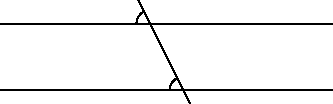
\includegraphics{euclid-I28}
\end{minipage}\\[10pt]

\noindent Up to this point, only the first four of Euclid's postulates are used. Thus in any model for which the first four postulates are true, it is possible to create parallel lines just by measuring angles. The parallel postulate (P5) is what tells us that, in Euclidean geometry, this is the \emph{only} way to create parallel lines.

\begin{thm*}[I.\,29]
Suppose that a line falls on two parallel lines. Then the alternate angles are equal.
\end{thm*}

\noindent This is precisely the \emph{converse} to Theorem I.\,27.

\noindent\begin{minipage}[t]{0.55\textwidth}\vspace{0pt}
\begin{proof}
We must prove that $\alpha=\beta$. Suppose not and WLOG that $\alpha>\beta$. But then $\beta+\gamma<\alpha+\gamma$ and so $\beta+\gamma$ is less than a straight edge. By the parallel postulate, the lines $\ell_1,\ell_2$ meet on the left side of the picture, whence $\ell_1$ and $\ell_2$ are not parallel.
\end{proof}
\end{minipage}\hfill
\begin{minipage}[t]{0.4\textwidth}\vspace{0pt}
\flushright\includegraphics{euclid-I29}
\end{minipage}

\paragraph{Angles in a triangle add to 180$^\circ$}

Finally, Euclid is in a position to prove the most famous result about triangles: that its interior angles sum to a straight edge. Euclid words this slightly differently.

\noindent\begin{minipage}[t]{0.55\textwidth}\vspace{0pt}
\begin{thm*}[I.\,32]
 If one side of a triangle is protruded, the exterior angle is equal to the two interior and opposite angles
\end{thm*}
\end{minipage}\hfill
\begin{minipage}[t]{0.4\textwidth}\vspace{0pt}
\flushright\includegraphics{geo-13-triangle}
\end{minipage}\\[10pt]

\noindent\begin{minipage}[t]{0.55\textwidth}\vspace{0pt}
\begin{proof}
\begin{enumerate}\itemsep0pt
  \item Construct $CE$ parallel to $BA$
	\item Then $\angle ABC=\angle ECD$ and\\
	$\angle ACE=\angle BAC$
	\item $\begin{array}{r@{\,}l}
	\\[-2pt]
	\therefore\angle ACD & =\angle ACE+\angle ECD\\
	&=\angle BAC+\angle ABC
	\end{array}$
\end{enumerate}
\end{proof}
\end{minipage}\hfill
\begin{minipage}[t]{0.4\textwidth}\vspace{0pt}
\flushright\includegraphics{geo-14-triangle2}
\end{minipage}
